8p\chapter{Preliminaries}
\label{chap:background}

% Describe what we need to understand to move forward
In this chapter, we discuss the preliminaries of encryption and quantum computation, the two ideas key to understanding the BB84 quantum KEP.


\section{Encryption}
Consider two parties, Alice and Bob, trying to communicate through a channel.
If the channel is insucure, a malicious third party, Eve, can listen and eavesdrop on the communication.
Encryption helps to make the communication more secure, by obscuring data such that an eavesdropper cannot gain any information by intercepting communication \cite{encrypt}.

\begin{figure}[htp]
\centering
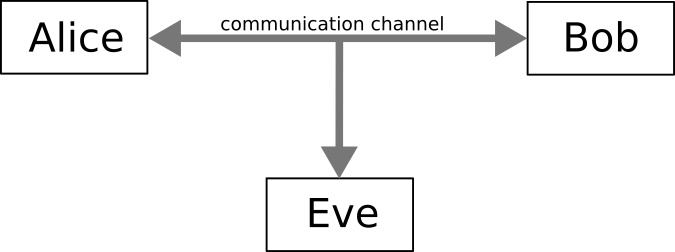
\includegraphics[scale=0.4]{images/classical_communication.png}
\caption{Alice and Bob communicate over an insecure channel with an eavesdropper, Eve}
\label{foo bar}
\end{figure}

In practice, information is encrypted by manipulating the data according to some encryption algorithm.
The goal of a good encryption algorithm is simple: allow the sender and receiver to access the information, but make the data useless to anyone else.
In order to allow for information to be decrypted by the receiver, the algorithm must be reversible with the use of a secret key, also known as the encryption key.
The basic encryption process is as follows:

\begin{itemize}
\item A sender, Alice, composes a message, referred to as the plaintext.
\item Alice encrypts the plaintext into cyphertext using some encryption algorithm and an encryption key.
\item Alice then sends the cyphertext to the receiver, Bob.
\item Bob uses the encryption key to decrypt the cyphertext into plaintext.
\item Note that the plaintext was never transmitted over the network.
\end{itemize}

Encryption appears in two general forms: symmetric and asymmetric, each with their own benefits and drawbacks. 


\subsection{Symmetric Encryption}
% Symmetric Encryption
Symmetric encryption is an encryption method in which both the sender and receiver, Alice and Bob respectively, use the same key.
\begin{figure}[htp]
\centering
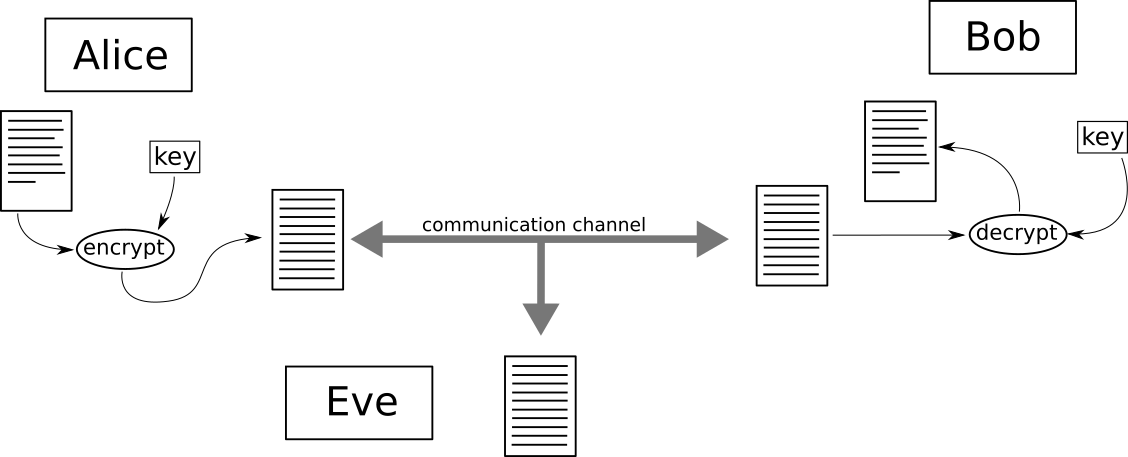
\includegraphics[scale=0.350]{images/symmetric_ecryption.png}
\caption{Alice and Bob symmetrically encrypt and decrypt a message}
\label{}
\end{figure}
While symmetric encryption is the oldest form of encryption, being used for over 4000 years, it does have a major drawback -- the key distribution problem: if Alice and Bob are separate parties (as in the case of secure message transmission), they must exchange their key beforehand using a secure channel \cite{cryptography}.
If an eavesdropper, Eve, were to intercept the key in transit, then the encryption is compromised and there is not necessarily any way for Alice or Bob to know.

% Talk about AES encryption and/or stream cyphers

% One Time Pad in depth
A One-Time-Pad (OTP) is a symmetric key that is used only once.
The OTP, as the name suggests, is discarded after a singe message has been sent, and the OTP is usually the same length as the message it encrypts.
This allows bit-wise encryption techniques, such as parity manipulation, to add the the security of the key and ensures that common frequency hacking techniques are not possible \cite{cryptography}.
In order to make the OTP truly secure, the bits used must be generated using a true-random number generator to avoid a malicious party guessing the pad.
Data is encrypted using a OTP with the following bitwise operation:
\begin{center}
\begin{tabular}{rc}
Plaintext: & $X = \{x_0, x_1, ..., x_n\}$ \\
OTP:  & $P = \{p_0, p_1, ..., p_n\}$  \\
Cyphertext:  & $Y = \{y_0, y_1, ..., y_n \}$\\
where  & $y_i = (x_i + p_i) \mod 2 $\\
\end{tabular}
\end{center}

For example, in binary:

\begin{center}
\begin{tabular}{rc}
Plaintext: &  \code{ 0 1 0 0 1 0 1 0} \\
OTP: &        \code{ 0 1 1 0 1 0 0 1} \\
Cyphertext: & \code{ 0 0 1 0 0 0 1 1} \\
\end{tabular}
\end{center}

To decrypt the cyphertext using the OTP, you simply apply the same opperation:

\begin{center}
\begin{tabular}{rc}
Cyphertext: & \code{ 0 0 1 0 0 0 1 1} \\
OTP: &        \code{ 0 1 1 0 1 0 0 1} \\
Plaintext: &  \code{ 0 1 0 0 1 0 1 0} \\
\end{tabular}
\end{center}
Under the proper conditions, a OTP is considered to be ``perfect encryption", and is only susceptible to brute force attacks, where one has to try every possible combination of the secret key, which is computationally infeasible \cite{cryptography}.
% One Time Pad caveats
However OTPs suffer from the same issue as all symmetric encryption protocols, the key distribution problem.
In the case of the OTP, not only does one encryption key have to be distributed, a unique key must be distributed for each message, making it highly impractical in most cases.

\subsection{Asymmetric Encryption}
% Asymmetric encryption
Asymmetric encryption, also known as public-key cryptography, on a classical computer, is the process of encrypting data using one key in such a way that it can be decrypted using a different key.
In effect, Alice can encrypt a message using a key that is publicly accessible, and the message can only be decrypted by Bob, who has the secret key corresponding to the public key used.
This method requires a key to be compromised of two parts, a public and private key-pair: $k = (k_{pub}, k_{priv})$ where $k_{pub} = f(k_{priv})$ \cite{cryptography}.

% Diffie Hellman in depth
The Diffie-Hellman KEP was the first asymmetric KEP to be proposed, and is still widely used in various forms today. 
It is performed as follows:

\begin{enumerate}
\item The sender and receiver, Alice and Bob respectively, establish a line of communication.
\item Some large prime $p$ and an integer $\alpha \in \{2,3,4,...,p-2\}$ are shared between Alice and Bob.
\item Alice and Bob each compute their own private keys, $a$ and $b$, respectively. $$k_{priv,A} = a \in \{2,3,4,...,p-2\}$$
\item Alice sends Bob her public key $A = \alpha^a \mod p$.
\item Bob sends Alice his public key $B = \alpha^b \mod p$. 
\item Alice computes a session key $k_{AB} = B^a \mod p$.
\item Bob computes a session key $k_{AB} = A^b \mod p$. 
Because $(\alpha^a)^b = (\alpha^b)^a = \alpha^{ab}$, both Alice and Bob's computations result in the same session key despite never knowing each other's private keys. 
\end{enumerate}

This method is cryptographically secure due to the Discreet Logarithm Problem (DLP), finding $x$ such that $B = \alpha^x \mod p$. 
This problem is computationally not feasible to solve using classical computers; although it has never been shown to be NP-Hard, nor has it been shown to be polynomial time solvable \cite{Shor_1997}.
Although these techniques are currently secure, they become easy to solve in the quantum space.

\section{Quantum Computation}

% Basic properties
Just as classical computation involves bits, quantum computation is computation using quantum bits, qubits, which are usually denoted using ``bra-ket" notation as $\ket{\psi}$ \cite{qc:agi}.
A ket is simply a representation of a vector, and in this case the vector is the ``state-vector" of the qubit, as further explained.
Similar to classical bits having the value 0 or 1, qubits' state can be the analogous $\ket{0}$ or $\ket{1}$.
These states will be used as binary, just like 0 and 1, for computation.
%	State
It is commonly said that while a classical bit exists in either the state 0 or 1, qubits can exist in both $\ket{0}$ and $\ket{1}$ at once.
There is an element of truth in this, but a more accurate description would be that as a qubits state-vector exists in a 3-dimensional space, and it can point somewhere in between the states $\ket{0}$ and $\ket{1}$. 
This state-vector is described as a linear combination $\ket{\psi} = \alpha\ket{0} + \beta\ket{1}$, where $|\alpha|^2 + |\beta|^2 = 1$, and $\alpha$ and $\beta$ are referred to as the amplitude of probability for their respective kets.

%	Measurement
Just as a computer can read the value of a classical bit, we can read, or``measure", a qubit.
The measurement is performed against two states, $\ket{0}$ and $\ket{1}$, and upon measurement the qubits state collapses to one of the two values.
The probability with which a vector will collapse into one of two states is the square of the amplitude for that state.
It is unknown exactly what causes the superposition to collapse, but it has been derived from empirical observations and is the single most important property of quantum mechanics \cite{qc:agi}.
For example, consider the qubit $\ket{\psi} = \frac{1}{\sqrt{3}}\ket{0} + \sqrt{\frac{2}{3}}\ket{1}$.
The probability that $\ket{\psi}$ will be $\ket{0}$ when measured is $(\frac{1}{\sqrt{3}})^2$, or $\frac{1}{3}$.
Any qubit or state-vector is defined using this vector formula.
If $\ket{\psi}$ is a linear combination of $\ket{0}$ and $\ket{1}$, and neither amplitudes are zero, the qubit is said to be in a superposition of $\ket{0}$ and $\ket{1}$.
Superposition is one of the fundamental properties of quantum computation \cite{qc:agi}. 

We use quantum operators called gates to manipulate $\alpha$ and $\beta$ probabilities.
For example, the Hadamard Gate, or H gate, performs what is called a "quarter turn"; it maps $$\ket{\psi} = \ket{0} \rightarrow \textSq{H} \rightarrow \ket{\psi} = \frac{1}{\sqrt{2}}\ket{0} + \frac{1}{\sqrt{2}}\ket{1}$$  $$\ket{\psi} = \ket{1} \rightarrow \textSq{H} \rightarrow \ket{\psi} = \frac{1}{\sqrt{2}}\ket{0} - \frac{1}{\sqrt{2}}\ket{1}$$ \cite{qc:agi}.
Since after the H gate is applied $\alpha$ and $\beta$ both equal $\frac{1}{\sqrt{2}}$, and ${(\frac{1}{\sqrt{2}})}^2 = \frac{1}{2}$, if we measure $\ket{\psi}$ in this state it would collapse to $\ket{0}$ and $\ket{1}$ with equal probability. 
It is worth noting this is one way to create a true-random number generator.

%	Bases
Because the state vector exists in a 3D state space, we do not necessarily have to measure against $\ket{0}$ and $\ket{1}$, in fact we can measure against any two vector values that are opposite each other on the unit circle. 
A set of vectors to measure against is known as a basis, and there are many possible bases. 
The set $\{\ket{0},\ket{1}\}$ is known as the standard basis or computational basis, as it is analogous to classical bits \cite{qcftgu}.
Another common basis is the Hadamard Basis, which is denoted $\ket{+} = \frac{1}{\sqrt{2}}\ket{0} + \frac{1}{\sqrt{2}}\ket{1}$ and $\ket{-} = \frac{1}{\sqrt{2}}\ket{0} - \frac{1}{\sqrt{2}}\ket{1}$.
The H gate will put $\ket{0} \rightarrow \ket{+}$ and $\ket{1} \rightarrow \ket{-}$, but it will also revert the Hadamard basis into the standard basis: $\ket{+} \rightarrow \ket{0}$ and $\ket{-} \rightarrow \ket{1}$.

Because the standard basis and the Hadamard basis are perpendicular to each other they are referred to as orthonormal bases.
That is to say if a $\ket{\psi} = \ket{+}$ or $\ket{\psi} = \ket{-}$ then it will have a 50\% change of being $\ket{0}$ or $\ket{1}$ if measured in the standard basis, and vice-versa \cite{qc:agi}. 

\begin{figure}[H]
\centering
\begin{tabular}{cc|cccc}
	&&\multicolumn{4}{|  c }{Measured value}  \\
	   &       &$ \ket{0}$ & $\ket{1}$ & $\ket{+}$ & $\ket{-}$\\ \hline
	\multirow{4}{*}{Qubit state} &$\ket{0}$ & $100\%$   & $0\%$     & $50\%$    &  $50\%$  \\
	&$\ket{1}$ & $0\%$     & $100\%$   & $50\%$    &  $50\%$  \\
	&$\ket{+}$ & $50\%$    & $50\%$    & $100\%$   &  $0\%$   \\
	&$\ket{-}$ & $50\%$    & $50\%$    & $0\%$     &  $100\%$ \\
\end{tabular}
\caption{The probability of measuring a qubit from one basis state into another}
\end{figure}

In effect, if you have a vector in one orthonormal basis it is useless if measured in another orthonormal basis.
Further, since the vector state changes when measured, if a value is encoded in one orthonormal basis, that information is destroyed by measuring in another orthonormal basis \cite{qcftgu}. 

% Guarantees
% 	Copy-ability
Another crucial property of qubits is that they cannot be cloned.
It is impossible to have an operator that clones the state of an input qubit into an output qubit without knowing the basis of the input \cite{qc:agi}.
This property proves crucial in the BB84 protocol, as explained in Chapter~\ref{chap:bb84}.

Using these properties and others, it has been shown that quantum computers can solve the DLP on an $n$-bit number in only $O(n^2\log n \log \log n)$ time \cite{MikeAndIke}.
Therefore, the popularity of quantum computers poses a serious threat to the securities of the Diffie Hellman KEP and asymmetric encryption.
The BB84 protocol is a quantum key distribution (QKD) protocol that allows two parties to co-create a shared key, using a verifiably secure channel, that can then be used to symmetrically encrypt messages.
